\chapter{Scaling and Convergence}
\label{chap:scaling_and_convergence}
The question of temporal convergence, as outlined in \sect{subsect:temporal_convergence}, is linked not only to the particular method used for approximating the temporal derivatives in , but also to the degree to which the nonlinearities are resolved over that time-step. 
In order to determine the degree to which a state vector, $\vec{x}$, satisfies \eqref{eqn:conservaton_equations}, the use of the nonlinear residual, $\vec{F}$, is required.
However, due to the formulation of the residual vector, the magnitudes of residuals can vary by orders of magnitude.
%--------------------------------------------------------------------------------------------------------------------------------------------------------------------
%--------------------------------------------------------------------------------------------------------------------------------------------------------------------
%--------------------------------------------------------------------------------------------------------------------------------------------------------------------
%--------------------------------------------------------------------------------------------------------------------------------------------------------------------
%--------------------------------------------------------------------------------------------------------------------------------------------------------------------
%--------------------------------------------------------------------------------------------------------------------------------------------------------------------
%--------------------------------------------------------------------------------------------------------------------------------------------------------------------

\section{Physics Based Scaling}
\label{sect:scaling}
For a given grid location, the nonlinear residuals for mass and energy, \eqref{eqn:cont_residual}, as formulated in section \ref{subsect:numerics_semi_implicit} will have six components.
These residuals will have the units of the conserved quantities for their corresponding PDEs.
Table \ref{tab:scaling_units_scales} shows some typical values of these conserved quantities during normal operations of typical PWR simulation.

\begin{table}[ht]
\centering
\begin{tabular}{|l|}
... your table ...
\end{tabular}
\caption{Typical scale for reactor simulations}
\label{tab:scaling_units_scales}
\end{table}

However, during accident scenarios, the range of these values can dramatically change.
One of the challenges that has been addressed during this work is coming up with a methodology for scaling that will provide a meaningful metric for convergence.
The scaling chosen should have the following characteristics:
\begin{itemize}
\item{$S^{-1}_k F(x_k)_i \approx 1$ when $x_k$ is a "poor" solution.}
\item{$S^{-1}_k F(x_k)_i \rightarrow 0$ when a phase disappears.}
\item{$0 \leq S^{-1}_k F(x_k)_i \leq 0 $ for all values of $F(x_k)_i$.}
\end{itemize}

The heart of the scaling used in this work is a physics-based methodology.
To illustrate the scaling procedure, we shall consider \eqref{eqn:conservation_of_liq} for a simply connected continuity cell without inter-field mass transfer.
Assume that the entire channel single phase and in thermodynamics equilibrium such that the macroscopic densities on either side of this single cell are the same.

\begin{equation}
F = \left(\alpha_k \rho_k\right)^{n+1} - \left( \alpha_k \rho_k \right)^n - \frac{\Delta t}{V} \left( \frac{\alpha_k \rho_k }{<\alpha_k \rho_k>^n} V^{n+1}_{j-1} \right)
\end{equation}

In this equation there are three physically meaningful quantities: the temporal difference, the mass flowing into the cell, and mass flowing out of the cell.
%--------------------------------------------------------------------------------------------------------------------------------------------------------------------
%--------------------------------------------------------------------------------------------------------------------------------------------------------------------
%--------------------------------------------------------------------------------------------------------------------------------------------------------------------
%--------------------------------------------------------------------------------------------------------------------------------------------------------------------
%--------------------------------------------------------------------------------------------------------------------------------------------------------------------
%--------------------------------------------------------------------------------------------------------------------------------------------------------------------
%--------------------------------------------------------------------------------------------------------------------------------------------------------------------

\section{Nonlinear Convergence vs. Temporal Convergence}
\label{sect:nonlinear_temporal_convergence}

Two test problems were constructed to examine the impact of nonlinear convergence on temporal convergence.
The primary purpose of the two problems studied is to determine the impact of resolving the nonlinearities at each time step for a given time-step size on the number of time-step size refinements necessary to reach a temporally converged solution.

\subsection{Geometry}
\label{subsect:experimental_geometry}
For both of the test problems, the same computational geometry was used; figure \ref{fig:exp_geometry} represents the experimental geometry.
Each block represents a single continuity cell with a height of 4 [in].
The total height of the channel is 48 [in].
Each continuity cell has a cross-sectional area of 4 [in$^2$] and a hydraulic diameter of 4 [in].
The red block at the top of the channel represents a boundary cell where the pressure and enthalpy are specified.
This boundary can be thought of an infinite reservoir filled with fluid at the specified conditions.
The red triangle represents a specified flow at the bottom edge of the 1st continuity cell. 
\begin{figure}[h!t]
\caption{Geometry for test problems.}
\label{fig:exp_geometry}
\begin{center}
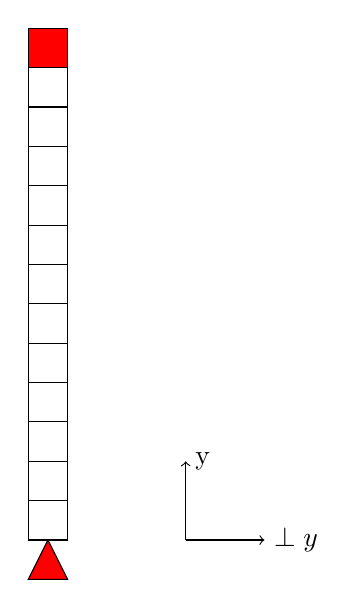
\begin{tikzpicture}
\foreach \x in {1,..., 12} \draw(0, 0.5*\x-0.5) rectangle +(.5,.5);
\filldraw[fill=red] (0, 6) rectangle +(.5,.5); 
\filldraw[fill=red] (0, -0.5) -- (0.25, 0) -- (0.5, -0.5) -- cycle;
\draw[->] (2,0) -- (2, 1) node[anchor=west] {y};
\draw[->] (2,0) -- (3, 0) node[anchor=west] {$\perp y$};
\end{tikzpicture}
\end{center}
\end{figure}

\subsection{Single Phase Flow in a Pipe}
\label{subsect:single_numerical_experiment}
The first problem examined was that of a stand-pipe filled with water.
There is an initial hydro-static head within the pipe.
The pressure-enthalpy boundary condition at the top of the channel has state properties equal to the initial state properties in the top continuity cell.
The specified inlet mass flow, $\dot{m}$, at the bottom of the channel is a time-dependent function give by \eqref{eqn:bc_time_func_single}.

\begin{equation}
\label{eqn:bc_time_func_single}
\dot{m}(t) = \left\{
\begin{array}{cclrcll}
 0.0           & [\frac{lb_m}{s}] & , &         & t & \leq 1 &[s] \\
 0.5 ( t - 1)  & [\frac{lb_m}{s}] & , & 1 [s] < & t & \leq 2 &[s] \\
 0.5           & [\frac{lb_m}{s}] & , &         & t & > 2    &[s]
\end{array}\right.
\end{equation}

Table \ref{tab:ic_single} provides the initial and boundary conditions for this problem.
The domain starts out at 100 [psia].

\begin{table}[h!t]
\centering
\begin{tabular}{|l|}
blarp
\end{tabular}
\caption{Initial and boundary conditions for single phase problem.}
\label{tab:ic_single}
\end{table}

\subsubsection{Results}
\label{subsubsect:single_results}
blarger!


\subsection{Superheated Liquid Flashing in a Pipe}
\label{subsect:flashing_numerical_experiment}

\subsubsection{Results}
\label{subsubsect:flashing_results}


\section{Review}
\label{sect:scaling_review}
